\section*{Tomás}
%
\section{Matrices de Weyl y sus propiedades} % {{{
Se definen las matrices de Weyl como:
\begin{align*}
U_{mn} = \sum_{k = 0}^{d-1} \omega_d^{km} |k\rangle \langle k \oplus n |,
\end{align*}
con $\omega_d = \exp(2\pi  i /d)$. Se pueden demostrar algunas propiedades de las matrices de Weyl, entre ellas se demuestra que:
\begin{align*}
U_{mn} U_{pq} U_{mn}^{\dagger} & = \sum_{k = 0}^{d-1} \omega_d^{km} |k\rangle \langle k \oplus n |   \sum_{j = 0}^{d-1} \omega_d^{jp} |j\rangle \langle j \oplus q |   \sum_{l = 0}^{d-1} \omega_d^{-lm} | l \oplus n\rangle \langle l| \\
& = \sum_{k,j,l=0}^{d-1} \omega_d^{km+jp-lm} |k \rangle \langle k \oplus n| j \rangle \langle j \oplus q | l \oplus n| \langle l | \\
& = \sum_{k,j,l=0}^{d-1} \omega_d^{km+jp-lm} \; \delta_{k\oplus n, j} \delta_{j\oplus q, l \oplus n} |k \rangle \langle l | \\
& = \sum_{k,l=0}^{d-1} \omega_d^{km + (k + n)p - lm} \delta_{k \oplus n \oplus q , l \oplus n} |k \rangle \langle l | \\
&= \sum_{k=0}^{d-1} \omega_d^{km + (k+n)p - (k+q)m} |k \rangle \langle k \oplus q | \\
& = \sum_{k=0}^{d-1} \omega_d^{np-mq} \sum_{k=0}^{d-1} \omega_d^{kp} |k \rangle \langle k \oplus q | \\
&=  \omega_d^{np-mq} U_{pq} 
\end{align*}
Es decir, concluimos que
\begin{align}
\label{conmutación matrices de Weyl}
U_{mn} U_{pq} U_{mn}^{\dagger}  = \omega_d^{np-mq} U_{pq} 
\end{align}

% }}}
\section{Mapas de Weyl y diagonalización} % {{{
En esta parte definimos los mapas de Weyl y los diagonalizamos. Es una forma diferente de probarlo y faltan algunos detalles, pero es al menos una comprobación de la diagonalización de Alejo y a lo mejor incluye ideas útiles. 

Para empezar, una matriz de densidad se puede escribir como
\begin{align}
\label{mat densidad}
\rho = \sum_{m,n=0}^{d-1} \alpha_{mn} U_{mn}
\end{align}
y un canal de Weyl se define como
\begin{align}
\label{forma de bloch}
\rho \rightarrow \rho' = \varepsilon(\rho) = \sum_{m,n = 0}^{d-1} \tau_{mn} \alpha_{mn} U_{mn}
\end{align}
Sin embargo, los canales de Weyl se pueden escribir de forma alternativa utilizando la forma de Kraus:
\begin{align}
\label{Forma de Kraus}
\varepsilon(\rho) = \sum_{m,n=0}^{d-1} k_{mn} U_{mn} \rho U_{mn}^{\dagger}.
\end{align}
Haría falta probar que efectivamente todos los canales de Weyl se pueden escribir así y que todos los canales escritos así son de Weyl, pero sé por lo menos que para el caso de qubits (canales de Pauli) se cumple. La ventaja de esta representación es que el canal es completamente positivo si y sólo si $k_{mn} \geq 0$ para toda $m,n$.

Entonces, buscamos ahora una relación entre  las $k$ y las $\tau$, para lo cual partimos de \ref{Forma de Kraus} y sustituimos la expresión de $\rho$:
\begin{align*}
\varepsilon(\rho) &= \sum_{m,n=0}^{d-1} k_{mn} U_{mn} \rho U_{mn}^{\dagger} = \sum_{m,n=0}^{d-1} k_{mn} U_{mn}  \sum_{p,q=0}^{d-1} \alpha_{pq} U_{pq} U_{mn}^{\dagger} \\ 
& = \sum_{m,n,p,q=0}^{d-1} k_{mn} \alpha_{pq} U_{mn} U_{pq} U_{mn}^{\dagger}  = \sum_{m,n,p,q=0}^{d-1} k_{mn} \alpha_{pq} \omega_d^{np-mq} U_{pq} \;\;\; \text{por (\ref{conmutación matrices de Weyl})} \\
& = \sum_{p,q=0}^{d-1} \left( \sum_{m,n=0}^{d-1} k_{mn} \omega_d^{np-mq} \right) \alpha_{pq} U_{pq}
\end{align*}
Vemos que el resultado vuelve a tener la forma de \ref{mat densidad}, pero con los componentes $\alpha_{pq}$ multiplicados por el término entre paréntesis, por lo que concluimos que este término es $\tau_{pq}$, es decir:
\begin{align}
\tau_{pq} = \sum_{m,n=0}^{d-1} k_{mn} \omega_d^{np-mq}
\end{align}
Esta expresión se puede voltear multiplicando ambos lados por $\omega_d^{lq-jp}$ y sumando sobre $p, q$, con lo que nos queda:
\begin{align*}
\sum_{p,q=0}^{d-1} \tau_{pq} \omega_d^{lq-jp} = \sum_{m,n,p,q=0}^{d-1} k_{mn} \omega_d^{np-mq} \omega_d^{lq-jp} = \sum_{m,n,p,q=0}^{d-1} k_{mn} \omega_d^{p(n-j)} \omega_d^{q(l-m)}
\end{align*}
La suma sobre $p$ se puede hacer usando que $\sum_p \omega_d^{p(n-j)} = d \delta_{nj}$ y similarmente sobre $q$ se usa que $\sum_q \omega_d^{q(l-m)} = d \delta_{lm}$.  Entonces nos queda que:
\begin{align*}
\sum_{p,q=0}^{d-1} \tau_{pq} \omega_d^{lq-jp} & = d^2 \sum_{m,n=0}^{d-1} k_{mn} \delta_{n,j} \delta_{l,m} = d^2 k_{lj}
\end{align*}
y concluimos que
\begin{align}
\label{k en terminos de lambda}
k_{lj} & =  \dfrac{1}{d^2} \sum_{p,q=0}^{d-1} \tau_{pq} \omega_d^{lq-jp} 
\end{align}
Vemos que este resultado difiere de las lambdas encontradas en la diagonalización de Alejo sólo por un factor de $d$.
Como las $k$ tienen que ser mayor o iguales a $0$ para que el canal sea completamente positivo y como las lambdas difieren de las $k$ sólo por un factor de $d$,  la conclusión sobre qué canales son válidos es la misma que cuando se hace la diagonalización. 


Regresamos ahora a la diagonalización obtenida por Alejo  y encontramos algunas otras ecuaciones que usaremos luego. Dicha diagonalización dice que:
\begin{align*}
\lambda_{kl} = \dfrac{1}{d} \sum_{\mu \nu = 0}^{d-1} \tau_{\mu \nu} \omega_d^{k \nu - \mu l}
\end{align*}
Esta expresión se puede voltear de forma similar a lo que se hizo para obtener \ref{k en terminos de lambda} y resulta que:
\begin{align}
\label{tau en termino de lambda}
\tau_{pq} = \dfrac{1}{d} \sum_{mn=0}^{d-1} \lambda_{mn} \omega_d^{pn-qm}
\end{align}
A partir de esta expresión, podemos hacer $p=q=0$, con lo que nos queda:
\begin{align*}
\tau_{00} = \dfrac{1}{d} \sum_{mn=0}^{d-1} \lambda_{mn} \omega_d^0,
\end{align*}
como $\tau_{00}=1$, concluimos que:
\begin{align}
\label{suma-lambdas}
\sum_{mn}^{d-1}\lambda_{mn} = d
\end{align}

% }}}
\section{Canales con $|\tau_{\mu\nu}|=1$ y propiedades algebráicas} % {{{

Vamos a definir canales parecidos a WCE pero generalizados para permitir
valores de $\tau$ distintos. 

\textbf{Definición, Canales con Multiplicadores de Norma Unitaria (Canales MNU):} Definimos un canal MNU
(o cambiar el nombre por uno mejor) como un canal de Weyl en el cual los
multiplicadores $\tau_{mn}$ cumplen que $|\tau_{mn}|= 1$.  Es decir, los
multiplicadores se encuentran en el círculo unitario. Notar que no incluyo por
ahora que $\tau_{mn} = 0$, pero a lo mejor se puede agregar luego. 
\cpnote{Será bueno ver que son estos canales con fases arbitrarias para qubits.}





\subsection{Propiedades de MNU}



\textbf{Teorema 1:} \textit{En un canal de Weyl, si $|\tau_{pq}| = 1$, entonces $\tau_{pq} = \omega_d^{k}$ para algún entero $k$. Por lo tanto, los únicos multiplicadores que hay que tomar en cuenta en canales MNU son los que sean raíces $d$-ésimas de la unidad.} \\

\textbf{Dem:} Partiendo de \ref{tau en termino de lambda}, tenemos que
\begin{align*}
& \tau_{pq} = \dfrac{1}{d} \sum_{mn=0}^{d-1} \lambda_{mn} \omega_d^{pn-qm} .
\end{align*}
Entonces, $\tau_{pq}$ es una suma convexa de varias raíces d-ésimas 
de la unidad (convexa porque la suma de los coeficientes $\lambda_{mn}/d$ es igual a $1$). 
Entonces, los posibles valores de $\tau_{pq}$ se encuentran 
en la envoltura convexa de estas raíces,
 lo cual forma un polígono regular de $d$ lados (y si además consideramos que $|\tau_{pq}|=1$, hay que considerar que cada $\tau$ se encuentra en el círculo unitario).
Este polígono intersecta al círculo unitario solamente en sus vértices,
 que son las raíces d-ésimas de la unidad.
 Por lo tanto, si $\tau_{pq}$ se encuentra en el círculo unitario, 
tiene que ser una raíz d-ésima de la unidad.  $ \blacksquare$  \\

Por lo tanto, en los canales MNU se puede considerar 
que los multiplicadores $\tau$ son siempre raíces de la unidad. \\

Con estos resultados podemos probar un lema que luego nos lleva a un teorema:\\




\textbf{Lema:} \textit{$\tau_{pq} = \omega_d^k$ (es decir, es una raíz $d$-ésima de la unidad) si  y sólo si $\lambda_{mn} = 0$ para todo $mn$ con $\omega_d^{pn-qm} \neq \omega_d^k$} \\

\textbf{Ida:}  Partiendo de \ref{tau en termino de lambda}, tenemos que:
\begin{align*}
& \omega_d^k = \tau_{pq}  \; \Rightarrow \; \omega_d^k = \dfrac{1}{d} \sum_{mn=0}^{d-1} \lambda_{mn} \omega_d^{pn-qm} \\
& \Rightarrow \; d = \sum_{mn=0}^{d-1} \lambda_{mn} \omega_d^{-k} \omega_d^{pn-qm} \\
& \Rightarrow \; 0 = \sum_{mn}^{d-1} \omega_d^{-k} \omega_d^{pn-qm} - \sum_{mn=0}^{d-1}\lambda_{mn} \;\; \text{por (\ref{suma-lambdas})} \\
& \Rightarrow \; 0 = \sum_{mn=0}^{d-1} \lambda_{mn} \left( \omega_d^{pn-qm-k} - 1 \right) 
\end{align*}
Como $\lambda_{mn} \geq 0$ para toda $mn$ (por completa positividad) y $\omega_d^{pn-qm-k} - 1$ tiene parte real menor o igual a $0$, entonces $\lambda_{mn} \left( \omega_d^{pn-qm-k} - 1 \right) $ tiene parte real menor o igual a $0$ y para que sumar sobre todas las $mn$ nos dé $0$, todos los sumandos tienen que ser $0$:
\begin{align*}
& \lambda_{mn} \left( \omega_d^{pn-qm-k} - 1 \right) = 0
\end{align*}
Entonces, si $\omega_d^{pn-qm-k} \neq 1$, se debe de tener que $\lambda_{mn} = 0$, que es lo que se quería probar. \\

\textbf{Regreso:} Consideramos que:
\begin{align*}
\tau_{pq}& = \dfrac{1}{d} \sum_{mn=0}^{d-1} \lambda_{mn} \omega_d^{pn-qm} \\
&= \dfrac{1}{d} \sum_{mn | \omega_d^{pn-qm} = \omega_d^k} \lambda_{mn} \omega_d^{pn-qm} +\dfrac{1}{d} \sum_{mn | \omega_d^{pn-qm} \neq \omega_d^k} \lambda_{mn} \omega_d^{pn-qm} \\
& = \dfrac{1}{d} \sum_{mn | \omega_d^{pn-qm} = \omega_d^k} \lambda_{mn} \omega_d^k + 0 \;\;\; \text{(por hipótesis, $ \lambda_{mn} = 0$ cuando $ \omega_d^{pn-qm} \neq \omega_d^k)$.} \\
& =  \dfrac{1}{d} \omega_d^k \sum_{mn | \omega_d^{pn-qm} = \omega_d^k} \lambda_{mn}
\end{align*}
Pero como las lambdas de la suma que quedan son las únicas distintas de $0$, la ecuación \ref{suma-lambdas} implica que esta suma es igual a $d$ y por lo tanto $\tau_{pq} = \omega_d^k$. $\blacksquare$ \\

\textbf{Teorema 2 (Propiedad algebráica):}  \textit{Si $\tau_{pq} = \omega_d^k$ y $\tau_{p'q'} = \omega_d^{k'}$ (es decir, tenemos que dos taus son raíces $d$-ésimas de la unidad), entonces se tiene que $\tau_{p \oplus p' , q \oplus q'} = \tau_{pq} \tau_{p'q'} = \omega_d^{k+k'}$.} \\

\textbf{Demostración:} Vamos a usar el regreso del lema, para lo que empezamos probando su hip\'otesis. Digamos que $\omega_d^{(p \oplus p') n - (q \oplus q')m} \neq \omega_d^{k+k'}$, lo que implica que $\omega_d^{p n - qm} \omega_d^{p'n - q'm} \neq \omega_d^{k+k'}$. \\
Para que se cumpla esto, se debe de tener que $ \omega_d^{p n - qm} \neq \omega_d^k$ o bien $\omega_d^{p'n-q'm} \neq \omega_d^{k'}$. \\

Si $\omega_d^{p n - qm} \neq \omega_d^k$ y como $\tau_{pq} = \omega_d^k$, la ida del lema implica que $\lambda_{mn} =0$. Por otro lado, si $\omega_d^{p'n-q'm} \neq \omega_d^{k'}$ y como $\tau_{p'q'} = \omega_d^{k'}$, la ida del lema implica que $\lambda_{mn} = 0$. En cualquier caso, concluimos que $\lambda_{mn} = 0$. \\

Entonces, hemos demostrado que $\omega_d^{(p \oplus p')n - (q\oplus q')m} \neq \omega_d^{k+k'}$ implica que $\lambda_{mn} = 0$, por lo que el regreso del lema implica que $\tau_{p \oplus p', q \oplus q'} = \omega_d^{k+k'}$ $\;\; \blacksquare$. \\

En particular, eso muestra que el conjunto de taus que valen 1 es cerrado bajo $\oplus$ (pues si $\tau_{pq}= 1$ y $\tau_{p'q'}=1$, el teorema dice que $\tau_{p\oplus p', q\oplus q'} = \tau_{pq} \tau_{p'q'} = 1$).  \\

Con este teorema se puede probar los canales MNU son justo los que se obtienen cuando las taus son las columnas de la matriz $a$ (generalizada al caso de $d$ niveles, donde se  puede definir como $a_{mnpq} = \omega_{d}^{np-mq}$ y después ``colapsarla'' a dos índices). Es decir, el siguiente teorema:\\

\textbf{Teorema 3:} \textit{Sólo hay $d^2$ canales MNU válidos. Cada uno consiste en una elección de taus de la forma $\tau_{pq} = \omega_d^{np-mq}$ (columnas de la matriz $a$) para alguna elección de $m,n$ de las $d^2$ posibles.}\\

Para probarlo, vemos primero que solamente hay $d^2$ canales MNU posibles. Para ver esto, notamos por el teorema 2 que si conocemos $\tau_{01}$ y $\tau_{10}$, todas las otras taus (y por tanto el canal completo) quedan determinadas. Esto debido a que cualquier $\tau_{pq}$ se va a poder calcular como productos de $\tau_{01}$ y $\tau_{10}$ usando la conclusión del teorema 2.  Como hay $d$ posibilidades para el valor de $\tau_{01}$ y de $\tau_{10}$, tenemos un total de a lo sumo  $d^2$ canales distintos. 

Por otro lado, se puede demostrar que si elegimos $\tau_{\mu\nu} = \omega_d^{m\nu-\mu n}$ para alguna elección de $m,n \in \{0,1, \cdots , d-1\}$ (es decir, alguna columna de $a$), entonces estas taus definen un canal válido. Para probarlo solamente hay que usar la diagonalización para esta elección de taus y ver que todas las lambdas son no negativas y reales:
\begin{align*}
\lambda_{kl} &= \dfrac{1}{d} \sum_{\mu \nu = 0}^{d-1} \tau_{\mu\nu} \omega_d^{k\nu-\mu l} \\
& = \dfrac{1}{d} \sum_{\mu \nu = 0}^{d-1} \omega_d^{m\nu-\mu n} \omega_d^{k\nu-\mu l} \\
& = \dfrac{1}{d} \sum_{\mu\nu = 0}^{d-1} \omega_d^{\nu (m+k)} \omega_d^{-\mu(\nu + l)}  \\
& = \dfrac{1}{d} \sum_{\mu=0}^{d-1} \omega_d^{-\mu(n + l)} \sum_{\nu=0}^{d-1} \omega_d^{\nu(m+k)} \\
&= \dfrac{1}{d} d \delta_{n,-l} d \delta_{m,-k} \;\;\; \text{Por propiedad que menciona alejo justo antes de la seccion 5}  \\
& = d \delta_{n,-l} \delta_{m,-k}
\end{align*}
Entonces, todas las lambdas son positivas, en particular, todas menos una valen $0$ y la otra (la de índices $(-m,-l)$) vale $d$.\\

Además, elecciones distintas de $m,n$ dan lugar a canales distintos, por lo que hemos encontrado $d^2$ canales distintos. 

Como vimos que hay a lo sumo $d^2$ canales MNU distintos y ya encontramos $d^2$ canales, concluimos que los canales MNU son exactamente esos. Es decir, los canales MNU son exactamente aquéllos de la forma $\tau_{pq}  =\omega_d^{np-mq}$ para las distintas elecciones de $m,n$. $\blacksquare$ \\ \\

A lo mejor hay una forma mejor de probar este resultado y sin necesidad del teorema 2. Y también puede ser que se pueda sacar una conclusión sobre una estructura interesante que tienen estos canales al usar el teorema 2. \\

Dejo aquí algunos dibujos de la matriz $a_{nmpq} = \omega_d^{np-mq}$ colapsada a dos dimensiones (en la horizontal el índice es $dm+n$ y en la vertical $dp+q$) para distintos valores de $d$. Cada entrada la pongo en un color desde el blanco para la raíz $\omega_d^0 = 1$ hasta negro para la última raíz $\omega_d^{d-1}$. Como se dijo antes, las columnas de esta matriz son los $d^2$ canales válidos, cada uno es $\tau_{pq} = \omega_d^{np-mq}$. 


\begin{figure}
    \centering
    \subfloat[\centering $d=2$]{{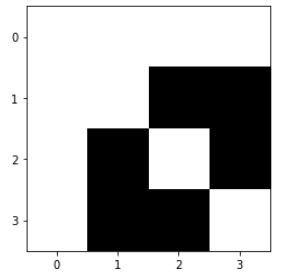
\includegraphics[width=5cm]{imagenes/d2.png} }}%
    \qquad
    \subfloat[\centering $d=4$]{{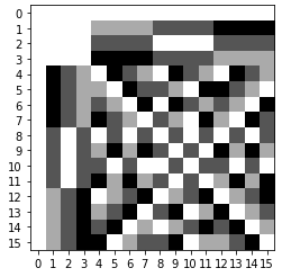
\includegraphics[width=5cm]{imagenes/d4.png} }} \\%
\centering
    \subfloat[\centering $d=10$]{{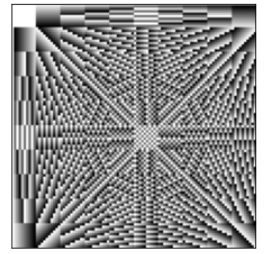
\includegraphics[width=5cm]{imagenes/d10.png} }}%
    \qquad
    \subfloat[\centering $d=12$]{{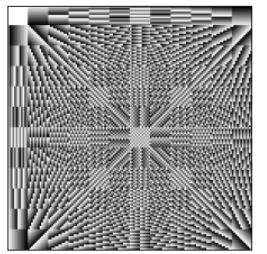
\includegraphics[width=5cm]{imagenes/d12.png} }}\\%
\centering
\subfloat[\centering $d=13$]{{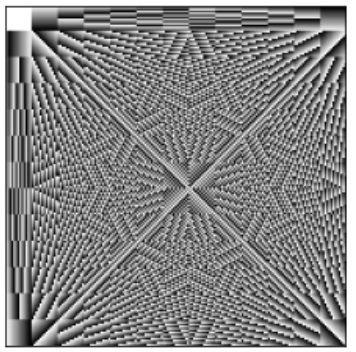
\includegraphics[width=5cm]{imagenes/d13.png} }}%
    \qquad
    \subfloat[\centering $d=17$]{{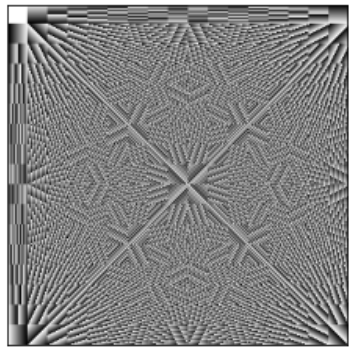
\includegraphics[width=5cm]{imagenes/d17.png} }}%
\end{figure}
% }}}
\newpage

\section{Las desigualdades}
Partimos de la diagonalización para tener las lambdas en términos de las taus:
\begin{align*}
\lambda_{kl} = \dfrac{1}{d} \sum_{\mu\nu=0}^{d-1} \tau_{\mu\nu} \omega_d^{k\nu - \mu l},
\end{align*}
y calculamos la parte real y la parte imaginaria de $\lambda_{kl}$,
considerando que las taus son complejas y se pueden separar en 
parte real e imaginaria como: $\tau_{\mu\nu} = \tau_{\mu\nu}^R + i \tau_{\mu\nu}^I$. 
La parte real de las lambdas la exigimos mayor o igual a $0$
 y la imaginaria 0 (para que las lambdas sean reales no negativos 
y el canal sea CP) y nos queda:
\begin{align}
Re(\lambda_{kl}) =  \sum_{\mu \nu} \left[ \cos \left( \dfrac{2\pi}{d}(k\nu-l\mu) \right) \tau_{\mu \nu}^R -\sin \left( \dfrac{2\pi}{d}(k\nu-l\mu) \right) \tau_{\mu \nu}^I \right] \geq 0 \label{desigualdades} \\
Im(\lambda_{kl}) = \sum_{\mu \nu} \left[ \cos \left( \dfrac{2\pi}{d}(k\nu-l\mu) \right) \tau_{\mu \nu}^I +\sin \left( \dfrac{2\pi}{d}(k\nu-l\mu) \right) \tau_{\mu \nu}^R \right] = 0.  \label{igualdades}
\end{align}
La cantidad de variables reales es $2d^2$ 
(o más bien $2d^2 - 2$ si consideramos que $\tau_{00} = 1$) y tenemos $d^2$ igualdades
y $d^2$ desigualdades. Por tanto, se deberían de poder usar las $d^2$ 
igualdades para reducir las $2d^2$
variables a $d^2$ y que las desigualdades sólo apliquen sobre ellas.

Para reducir las variables, primero definiremos dos conjuntos de vértices como siguen (se supone siempre la suma módulo $d$):

\begin{align*}
Inv &= \{(\mu,\nu)\; | ;\ (\mu , \nu) = (d-\mu, d-\nu)\},
\end{align*}
es decir, $Inv$ son los índices $(\mu,\nu)$ que son sus propios inversos bajo la suma módulo $d$. 
Luego, todos los índices restantes (los que no están en $Ainv$) se pueden arreglar en parejas de cada elemento y su inverso. Es decir, cada vértices  de los restantes como $(\mu,\nu)$ tiene emparejado su inverso $(d-\mu,d-\nu)$ (que es distinto a $(\mu,\nu)$). 

Entonces, definimos un conjunto $B$ como un conjunto de  índices que toma un solo índice de cada una de estas parejas de elemento e inverso. Definimos $B^{-1}$ como el los inversos de los elementos de $B$. \\

\textbf{Ejemplo:}
\begin{itemize}
\item $d=3$: Para qutrits, todos los índices son $\{(0,0), (0,1), (0,2), (1,0) ,(1,1), (1,2), (2,0), (2,1), (2,2) \}$. Entonces, $Inv = \{(0,0)\}$. El resto de los elementos se dividen en $4$ parejas de elemento - inverso de la forma $\{(0,1), (0,2)\} \; ,\; \{(1,0), (2,0)\} \; ,\; \{(1,1), (2,2)\} \; ,\; \{(1,2) , (2,1)\}$. Para elegir $B$, seleccionamos uno de los elementos de cada pareja (arbitrariamente), como por ejemplo: $B = \{(0,1), (1,0), (1,1) ,(1,2)\}$ y entonces $B^{-1} = \{(0,2), (2,0), (2,2), (2,1)\}$.\\

\item $d=4$: Para qutrits, todos los índices son $\{(0,0), (0,1), (0,2),(0,3), (1,0) ,(1,1), (1,2),(1,3)$, $(2,0), (2,1), (2,2),(2,3) , (3,0), (3,1),(3,2), (3,3) \}$. Entonces, $Inv = \{(0,0), (0,2), (2,0), (2,2)\}$. El resto de los elementos se dividen en $6$ parejas de elemento - inverso de la forma \\
$\{(0,1), (0,3)\} \; ,\; \{(1,0), (3,0)\} \; ,\; \{(1,1), (3,3)\} \; ,\; \{(1,2) , (3,2)\} \;$ ,$\; \{(1,3) , (3,1)\} \; ,\; \{(2,1), (2,3)\}$. \\
Para elegir $B$, seleccionamos uno de los elementos de cada pareja (arbitrariamente), como por ejemplo: $B = \{(0,1), (1,0), (1,1) ,(1,2), (1,3), (2,1)\}$ y entonces \\
$B^{-1} = \{(0,3) ,(3,0),(3,3),(3,2),(3,1),(2,3)\}$. \\
\item Notar que en general si $d$ es par, entonces $Inv = \{ (0,0) , (0,d/2), (d/2,0), (d/2,d/2)\}$ y $B$ tiene la mitad de los $d^2-4$ elementos restantes. Si $d$ es impar, entonces $Inv = \{(0,0)\}$ y $B$ tiene la mitad de los $d^2 - 1$ elementos restantes. 
\end{itemize}
\textbf{Teorema 4:} \textit{Las $d^2$ igualdades \ref{igualdades} son equivalentes a las $d^2$ igualdades siguientes:}
\begin{align}
\tau_{\mu \nu}^R = \tau_{d-\mu, d-\nu}^R \;\;\;\; ,\;\; \text{para $(\mu,\nu) \in B$}
\label{ecs Re} \\
\tau_{\mu \nu}^I = - \tau^I_{d-\mu, d-\nu} \;\;\;\;,\;\; \text{para $(\mu , \nu) \in B \cup Inv $}
\label{ecs Im}
\end{align}
\textit{(notar que son efectivamente $d^2$ igualdades)}. \\

\textbf{Dem:} Partiremos de las igualdades \ref{ecs Re} , \ref{ecs Im} y llegaremos a las igualdades \ref{igualdades}.
Empezamos multiplicando las ecuaciones \ref{ecs Re} por $\sin\left( \dfrac{2\pi}{d}(k\nu - l \mu)\right)$ 
y las \ref{ecs Im} por $\cos\left( \dfrac{2\pi}{d}(k\nu - l \mu)\right)$.
Entonces nos queda:
\begin{align*}
\sin\left( \dfrac{2\pi}{d}(k\nu - l \mu)\right) \tau_{\mu\nu}^R = \sin\left( \dfrac{2\pi}{d}(k\nu - l \mu)\right) \tau_{d-\mu, d-\nu}^R \;\;\; ,\; (\mu,\nu) \in B \\
\cos\left( \dfrac{2\pi}{d}(k\nu - l \mu)\right) \tau_{\mu\nu}^I = -\cos\left( \dfrac{2\pi}{d}(k\nu - l \mu)\right) \tau_{d-\mu, d-\nu}^R \;\;\; ,\; (\mu,\nu) \in B \cup Inv 
\end{align*}
Despejamos cada una de estas ecuaciones y las sumamos sobre $B$:
\begin{align*}
\sum_{(\mu,\nu) \in B} \left[  \sin\left( \dfrac{2\pi}{d}(k\nu - l \mu)\right) \tau_{\mu\nu}^R - \sin\left( \dfrac{2\pi}{d}(k\nu - l \mu)\right) \tau_{d-\mu, d-\nu}^R\right] = 0 \\
\sum_{(\mu,\nu) \in B}\left[ \cos\left( \dfrac{2\pi}{d}(k\nu - l \mu)\right) \tau_{\mu\nu}^I + \cos\left( \dfrac{2\pi}{d}(k\nu - l \mu)\right) \tau_{d-\mu, d-\nu}^I \right] = 0
\end{align*}
Luego, utilizamos que $\sin \left( \dfrac{2\pi}{d}(k(d-\nu) - l(d-\mu)) \right) = -\sin \left( \dfrac{2\pi}{d}(k\nu - l\mu) \right)$ (usando que $\sin(x + 2\pi n) = \sin(x)$ y que $\sin (-x) = -\sin(x)$). \\
También usamos que $\cos \left( \dfrac{2\pi}{d}(k(d-\nu) - l(d-\mu)) \right) = \cos \left( \dfrac{2\pi}{d}(k\nu - l\mu) \right)$ y nos quedan:
\begin{align*}
\sum_{(\mu,\nu) \in B}\left[  \sin\left( \dfrac{2\pi}{d}(k\nu - l \mu)\right) \tau_{\mu\nu}^R + \sin\left( \dfrac{2\pi}{d}(k(d-\nu) - l (d-\mu))\right) \tau_{d-\mu, d-\nu}^R \right] = 0 \\
\sum_{(\mu,\nu) \in B} \left[ \cos\left( \dfrac{2\pi}{d}(k\nu - l \mu)\right) \tau_{\mu\nu}^I + \cos\left( \dfrac{2\pi}{d}(k(d-\nu) - l (d-\mu))\right) \tau_{d-\mu, d-\nu}^I\right]  = 0
\end{align*}
Pero se tiene que $\sum_{(\mu,\nu) \in B} \sin\left( \dfrac{2\pi}{d}(k(d-\nu) - l (d-\mu))\right) \tau_{d-\mu, d-\nu}^R = \sum_{(\mu,\nu)\in B^{-1}} \sin\left( \dfrac{2\pi}{d}(k\nu - l \mu)\right) \tau_{\mu\nu}^R$ y similarmente para coseno, por lo que nos queda:
\begin{align*}
\sum_{(\mu,\nu) \in B}  \sin\left( \dfrac{2\pi}{d}(k\nu - l \mu)\right) \tau_{\mu\nu}^R + \sum_{(\mu,\nu) \in B^{-1}} \sin\left( \dfrac{2\pi}{d}(k\nu - l \mu)\right) \tau_{\mu\nu}^R  = 0 \\
\sum_{(\mu,\nu) \in B} \cos\left( \dfrac{2\pi}{d}(k\nu - l \mu)\right) \tau_{\mu\nu}^I + \sum_{(\mu,\nu) \in B^{-1}} \cos\left( \dfrac{2\pi}{d}(k\nu - l \mu)\right) \tau_{\mu\nu}^I  = 0
\end{align*}
Finalmente, notamos que si $(\mu,\nu) \in Inv$, entonces $\sin\left( \dfrac{2\pi}{d}(k\nu - l \mu) \right) = 0$,
lo que implica trivialmente que $\sum_{(\mu,\nu) \in Inv} \sin\left( \dfrac{2\pi}{d}(k\nu - l \mu) \right)  \tau_{\mu \nu}^R = 0$.
Además, por \ref{ecs Im}, se cumple que si $(\mu,\nu) \in Inv$, 
entonces $\tau_{\mu\nu}^I = -\tau_{d-\mu,d-\nu}^I$ 
y entonces $\tau_{\mu\nu}^I = 0$, lo que implica trivialmente 
que $\sum_{(\mu,\nu) \in Inv} \cos\left( \dfrac{2\pi}{d}(k\nu - l \mu)\right) \tau_{\mu\nu}^I  = 0$. 
Podemos agregar estos dos resultados a las ecuaciones que teníamos:
\begin{align*}
\sum_{(\mu,\nu) \in B}  \sin\left( \dfrac{2\pi}{d}(k\nu - l \mu)\right) \tau_{\mu\nu}^R + \sum_{(\mu,\nu) \in B^{-1}} \sin\left( \dfrac{2\pi}{d}(k\nu - l \mu)\right) \tau_{\mu\nu}^R  + \sum_{(\mu,\nu) \in Inv} \sin\left( \dfrac{2\pi}{d}(k\nu - l \mu) \right)  \tau_{\mu \nu}^R  = 0 \\
\sum_{(\mu,\nu) \in B} \cos\left( \dfrac{2\pi}{d}(k\nu - l \mu)\right) \tau_{\mu\nu}^I + \sum_{(\mu,\nu) \in B^{-1}} \cos\left( \dfrac{2\pi}{d}(k\nu - l \mu)\right) \tau_{\mu\nu}^I  + \sum_{(\mu,\nu) \in Inv} \cos\left( \dfrac{2\pi}{d}(k\nu - l \mu) \right) \tau_{\mu \nu}^I = 0
\end{align*} 
Pero en cada una de estas ecuaciones estamos ya sumando sobre todos los índices, que son $Inv \cup B \cup B^{-1}$ 
y entonces:
\begin{align*}
\sum_{\mu,\nu}\sin\left( \dfrac{2\pi}{d}(k\nu - l \mu)\right) \tau_{\mu\nu}^R  = 0 \\
\sum_{\mu,\nu} \cos\left( \dfrac{2\pi}{d}(k\nu - l \mu)\right) \tau_{\mu\nu}^I =0  
\end{align*}
Y sumando ambas nos queda:
\begin{align*}
\sum_{\mu\nu} \sin\left( \dfrac{2\pi}{d}(k\nu - l \mu)\right) \tau_{\mu\nu}^R+ \cos\left( \dfrac{2\pi}{d}(k\nu - l \mu)\right) \tau_{\mu\nu}^I = 0,
\end{align*}
que son las igualdades \ref{igualdades}. Con ello probamos que es posible pasar de \ref{ecs Im}, \ref{ecs Re} a las igualdades \ref{igualdades} con sólo multiplicar las ecs \ref{ecs Im},\ref{ecs Re} por constantes y sumando. Esto prueba que los dos sistemas de ecuaciones son equivalentes. $\blacksquare$ \\ \\ \\

Luego, sabiendo que las igualdades que teníamos en \ref{igualdades} son equivalentes a \ref{ecs Im}, \ref{ecs Re}, podemos usar éstas últimas para simplificar las variables.

Notamos primero que \ref{ecs Im} implica que si $(\mu,\nu) \in Inv$, entonces $\tau_{\mu\nu}^I = - \tau_{d-\mu, d-\nu}^I = -\tau_{\mu,\nu}^I$ y entonces $\tau_{\mu,\nu}^I = 0$. Es decir, los elementos $\tau_{\mu,\nu}$ para $(\mu,\nu) \in Inv$ son reales puros. 
Además, vemos de \ref{ecs Im}, \ref{ecs Re} que si conocemos $\tau_{\mu\nu}^R , \tau_{\mu \nu}^I$ para $(\mu,\nu)\in B$, entonces podemos conseguir $\tau_{(d-\mu,d-\nu)}^R , \tau_{(d-\mu,d-\nu)}^I$. Esto implica que las únicas variables libres son $\tau_{\mu\nu}^R$ para $(\mu,\nu) \in Inv$ y $\tau_{\mu\nu}^R, \tau_{\mu\nu}^I$ para $(\mu,\nu) \in B$. \\

Luego, usando las igualdades \ref{ecs Im}, \ref{ecs Re}, se pueden reescribir las desigualdades \ref{desigualdades} pero para que ahora solamente dependan de las variables libres y queda como:
\begin{align*}
\boxed{\sum_{(\mu,\nu)\in B} 2 \cos \left( \dfrac{2\pi}{d}(k\nu - l\mu) \right) \tau_{\mu\nu}^R + \sum_{(\mu,\nu)\in Inv} \cos \left( \dfrac{2\pi}{d}(k\nu - l\mu) \tau_{\mu\nu}^R + \sum_{(\mu,\nu)\in B} 2 \sin \left( \dfrac{2\pi}{d}(k\nu - l\mu) \tau_{\mu\nu}^I \geq 0}
\end{align*}

\section*{Politopo}


\begin{itemize}
\item Al final de la sección anterior nos quedaron $d^2$ desigualdades para $d^2-1$ variables libres (son $d^2-1$ variables libres si consideramos que $\tau_{00} = 1$, ya que entonces $\tau_{00}^R = 1$ y no es libre). 
\item Estas desigualdades definen un politopo formado por la intersección de $d^2$ hiperplanos en un espacio de $d^2-1$ dimensiones. 
\item Usando las desigualdades, se pueden encontrar los vértices de este politopo para las variables libres. Luego, se pueden usar las igualdades \ref{ecs Im}, \ref{ecs Re} para recuperar también las variables dependientes y conseguir así los canales todas las taus complejas que definen al canal del vértice. \\

Eso justo hicimos para $d=3,4$ computacionalmente y encontramos que los vértices son las columnas de la matriz $a$. \\

\item\textbf{Teorema:} \textit{Eso nos lleva a demostrar que en general los vértices del politopo de canales de weyl para qudits son justo las columnas de $a$}: \\

\textbf{Dem:} Empezamos demostrando lo siguiente:

\item \textbf{Las taus de un canal de Weyl  no pueden tener magnitud mayor a $1$:} Partimos de \ref{tau en termino de lambda}, que dice que:
\begin{align*}
\tau_{pq} = \dfrac{1}{d} \sum_{mn=0}^{d-1} \lambda_{mn} \omega_d^{pn-qm}.
\end{align*}
Entonces $\tau_{pq}$ es una suma convexa de varias raíces d-ésimas de la unidad
(convexa porque la suma de $\lambda_{mn}/d $ es $1$). 
Por lo tanto, los posibles valores de $\tau$ se encuentran en la envoltura convexa
 de estas raíces. Dicha envoltura convexa tiene como vértices a las raíces de la unidad 
 (o a lo mejor sólo algunas de las raíces de la unidad).
 Luego, $\tau_{pq}$ no puede tener norma mayor que $1$, pues saldría de esta envoltura convexa.  \\
 
Esto prueba que el politopo de canales de Weyl no puede incluir taus con norma mayor que $1$, pues ya no son canales.
 
\item \textbf{Los canales MNU (que son columnas de la $a$) son vértices del politpo:} 
Como las taus no pueden tener magnitud mayor a $1$, 
los canales en las que todas las taus tienen magnitud igual a $1$ 
(canales MNU) están en la frontera del politopo
(pues, si aumentamos tantito alguna de las taus, 
se salen del politopo de canales válidos por tener una tau de magnitud mayor que $1$). \\
 
\item \textbf{Los vértices del politopo son los canales MNU (y por tanto son las columnas de la $a$):} 
Para el politopo tenemos un total de $d^2$ desigualdades que lo definen y con $d^2 - 1$ variables libres. Entonces, a lo mucho habrá $d^2$ vértices. Como ya encontramos $d^2$ vértices en el inciso anterior, concluimos que estos tienen que ser todos los vértices del politopo.
\end{itemize}